\begin{comment}
  \section*{Math 202a - HW1 - Dan Davison - \texttt{ddavison@berkeley.edu}}

  \begin{mdframed}
    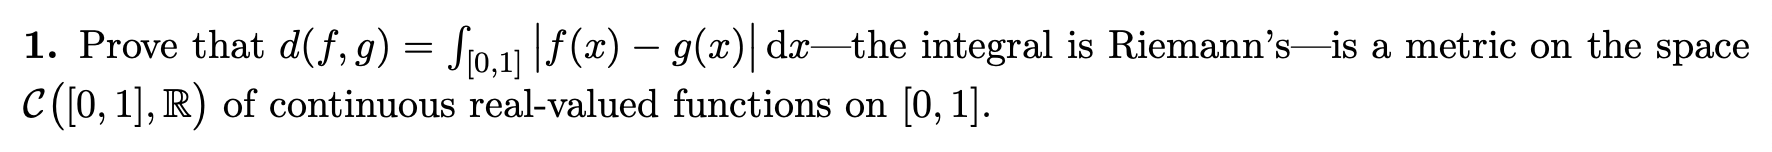
\includegraphics[width=400pt]{img/analysis--berkeley-202a--homework-1-a75a.png}
  \end{mdframed}


  \begin{proof}
    $d$ is a metric if it satisfies (I) $d(f,f) = 0$, (II) $d(f,g) = d(g, f)$, and (III) $d(f,g) + d(g, h) \le d(f, h)$.

    (I) is satisfied: $d(f, f) = \int_{[0,1]}|f(x) - f(x)| \dx = 0$.

    (II) is satisfied:
    \begin{align*}
      d(f, g)
      &= \int_{[0,1]}|f(x) - g(x)| \dx \\
      &= \int_{[0,1]}|g(x) - f(x)| \dx \\
      &= d(g, f),
    \end{align*}

    (III) is satisfied:
    \begin{align*}
      d(f, g) + d(g, h)
      &= \int_{[0,1]} |f(x) - g(x)| \dx + \int_{[0,1]} |g(x) - h(x)| \dx \\
      &= \int_{[0,1]} |f(x) - g(x)| + |g(x) - h(x)| \dx \\
      &\le \int_{[0,1]} |f(x) - g(x) + g(x) - h(x)| \dx \\
      &= \int_{[0,1]} |f(x) - h(x)| \dx \\
      &= d(f, h).
    \end{align*}
  \end{proof}

  \newpage
  \begin{mdframed}
    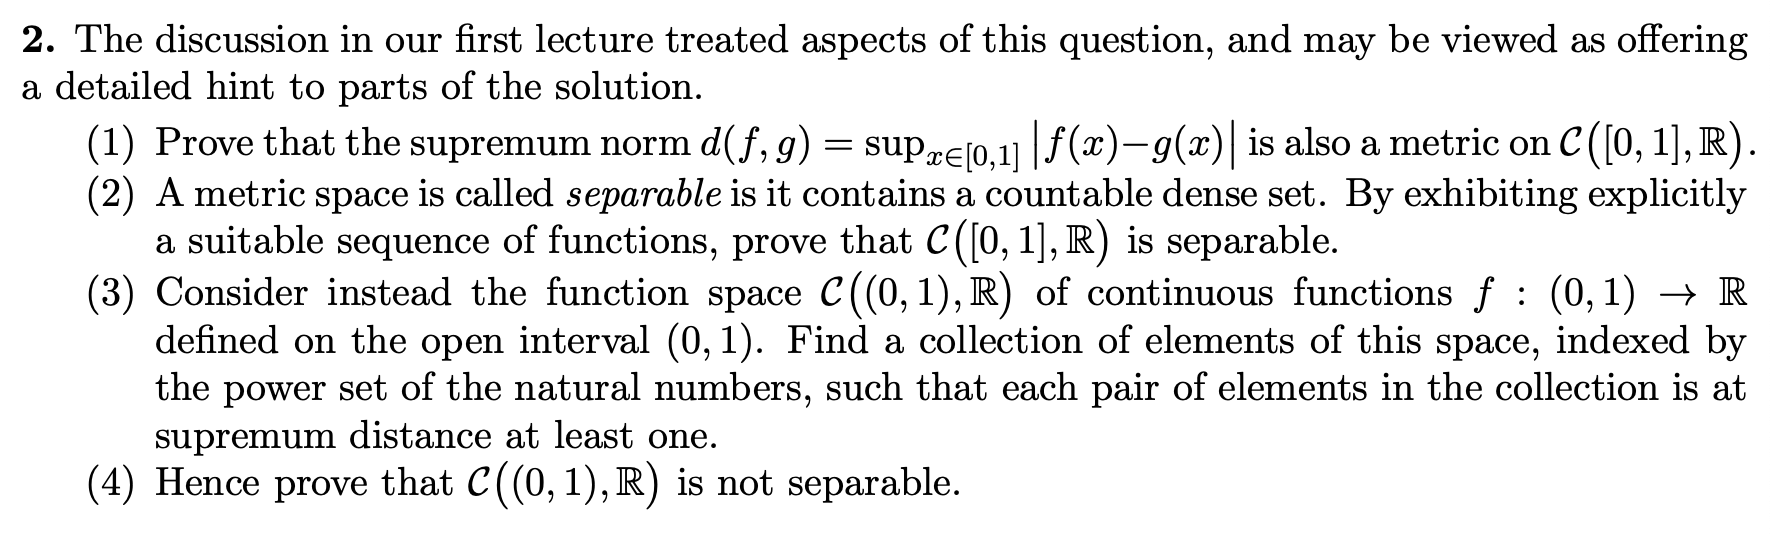
\includegraphics[width=400pt]{img/analysis--berkeley-202a--homework-1-d1d3.png}
  \end{mdframed}

  \begin{enumerate}
  \item
    \begin{proof}
      $d$ is a metric on the function space $\mathcal C\([0, 1], \R\)$ if it satisfies (I) $d(f,f) = 0$,
      (II) $d(f,g) = d(g, f)$, and (III) $d(f,g) + d(g, h) \le d(f, h)$.

      (I) is satisfied: $\sup_{x\in [0,1]} |f(x) - f(x)| = \sup_{x\in [0,1]} 0 = 0$.

      (II) is satisfied:
      \begin{align*}
        d(f, g)
        &= \sup_{x \in [0,1]}|f(x) - g(x)| \\
        &= \sup_{x \in [0,1]}|g(x) - f(x)| \\
        &= d(g, f),
      \end{align*}
      (III) is satisfied:
      \begin{align*}
        d(f, g) + d(g, h)
        &=   \sup_{x \in [0,1]} |f(x) - g(x)| + \sup_{x \in [0,1]} |g(x) - h(x)| \\
        &=   \sup_{x \in [0,1]} \Big(|f(x) - g(x)| + |g(x) - h(x)|\Big) \\
        &\le \sup_{x \in [0,1]} |f(x) - h(x)| \\
        &=   d(f, h).
      \end{align*}
    \end{proof}
  \item
    \begin{claim*}
      $\mc C\([0, 1], \R\)$ is separable.
    \end{claim*}

    \begin{proof}
      Let $\mc C$ be the set of continuous functions $[0, 1] \to \R$.

      Fix an arbitrary function $f \in \mc C$ and fix some $\epsilon > 0$.

      Define $g^*_n: [0, 1] \to \R$ as follows:
      \begin{enumerate}
      \item For all $i \in 0, 1, 2, \ldots, n$ set $x_i = i/n$.
      \item For all $i \in \{0, 1, 2, \ldots, n\}$, set $y^*_i = f(x_i)$. (Note that $y^*_i$ is in general not a rational
        number; we will account for this later.)
      \item For all $i \in \{1, 2, \ldots, n\}$ draw a straight line segment connecting $(x_{i-1}, y^*_{i-1})$
        and $(x_i, y^*_i)$.
      \item Define $g^*_n: [0, 1] \to \R$ to be the function whose graph was just drawn. (It is possible to give an
        explicit procedure for computing $g^*_n(x)$ by finding the interval in which $x$ lies and then using linear
        interpolation.)
      \end{enumerate}

      We now modify the definition of the family of approximating functions so that the $y$-coordinates of the
      endpoints are rational. Define $g_n: [0, 1] \to \R$ as follows:
      \begin{enumerate}
      \item Construct the sets of points $\{(x_i, y^*_i) ~|~ i \in \{0, 1, 2, \ldots, n\}\}$ as above.
      \item For $i \in \{0, 1, 2, \ldots, n\}$ set $y_i$ equal to a rational number in the
        interval $(y^*_i - \epsilon/4, y^*_i)$. (Such a rational number exists: for example, set $k$ equal to the
        smallest natural number such that $1/k < \epsilon/4$, and then set $j$ equal to the smallest natural number
        such that $j/k > y^*_i - \epsilon/4$. Then $j/k$ is a rational number in $(y^*_i - \epsilon/4, y^*_i)$.)
      \item For all $i \in \{1, 2, \ldots, n\}$ draw a straight line segment connecting $(x_{i-1}, y_{i-1})$
        and $(x_i, y_i)$.
      \item Define $g_n: [0, 1] \to \R$ to be the function whose graph was just drawn.
      \end{enumerate}
      Note that, since $f$ is continuous on a compact domain, $f$ is uniformly continuous. Fix some $\delta > 0$ such
      that $|x - x'| < \delta \implies |f(x) - f(x')| < \epsilon$ for all $(x, x') \in [0, 1]^2$.

      Set $m$ equal to the smallest natural number such that $1/m < \delta/2$ and note
      that $|f(x) - g_n(x)| < \epsilon$ for all $x \in [0, 1]$ due to the uniform continuity of $f$. (Informally,
      this is true because we can view uniform continuity as stating that a rectangle of base $\delta$ and
      height $\epsilon$ can be positioned over the graph at any point such that the graph intersects the left and
      right edges of the rectange but does not otherwise leave the rectangle. Our piecewise affine function
      consists of straight line segments that fit within such rectangles.) Therefore $d(g_n, f) < \epsilon$ for
      all $n \geq m$ and so $\{g_n | n \in \N\}$ is dense in $\mc C$.

      Finally we must show that $\{g_n ~|~ n \in \N\}$ is countable. Note that $g_n$ is piecewise affine for a
      given $n$, and that the $x$-coordinates of the endpoints are fixed. Thus for a given $n$, the cardinality
      of $\{g_n\}$ is equal to the cardinality of the set of possible $y$-coordinates. The latter set is $\Q^n$.
      Thus the cardinality of $\{g_n ~|~ n \in \N\}$ is equal to the cardinality of the
      set $\bigcup_{n\in \N} \Q^n$. This is a countable union of countable sets and is therefore countable.
    \end{proof}

  \item
    \begin{proof}
      Let $f_s: (0, 1) \to \R$ be given by $f_s(x) = \frac{1}{r(s)x}$, where $s \in 2^\N$ and $r(s) \in [0, 1]$ is
      the real number corresponding to $s$, i.e. the number $r(s) = 0.d_1d_2d_3\ldots$ where
      \begin{align*}
        d_i =
        \begin{cases}
          1, ~~~~ \text{if} ~~~~ i \in s,\\
          0, ~~~~ \text{otherwise}.
        \end{cases}
      \end{align*}
      Note that for real $a, b$ we have
      \begin{align*}
        \frac{1}{ax} - \frac{1}{bx} = \frac{b - a}{abx}
      \end{align*}
      and therefore the supremum distance between any two elements $f_{s_1}$ and $f_{s_2}$ is unbounded
      as $x \to 0$.
    \end{proof}
  \item
    \begin{proof}
      Let $\mc C$ be the set of continuous functions $f: (0, 1) \to \R$.

      Assume for a contradiction that $\mc C$ is separable. Let $\mc G \subset \mc C$ be a countable dense set of
      functions.

      Recall that in part (3) we found an uncountable set $\mc H \subset \mc C$ with the property that every pair
      of elements in $\mc H$ is at supremum distance at least one.

      But this is a contradiction, since we can establish a bijection between $\mc H$ and $\mc G$ as follows:

      Pick an element $h_1 \in \mc H$. Since $\mc G$ is dense in $\mc C$, there exists $g_1 \in \mc G$ such
      that $d(h_1, g_1) < 1/2$. Now pick $h_2 \in \mc H$ such that $h_1 \neq h_2$. Again, there
      exists $g_2 \in \mc G$ such that $d(h_2, g_2) < 1/2$. Furthermore, by the triangle
      inequality, $g_2 \neq g_1$. Continuing in this fashion, on the $i$-th iteration we pick $h_i \in \mc H$ and
      find a nearby $g_i \in \mc G$ such that $d(h_i, g_i) < 1/2$, and by the triangle inequality conclude
      that $g_i \neq g_j$ for all $j < i$.

      Thus we can associate each element of $\mc H$ with a unique element of $\mc G$ and conclude that the
      cardinality of $\mc G$ equals that of $\mc H$, which is that of the power set of the natural numbers.
      But $\mc G$ is countable; a contradiction. Therefore no such countable dense set $\mc G$ exists and $\mc C$
      is not separable.
    \end{proof}


    But can find bounded fns with image [0, 1]

    \begin{mdframed}
      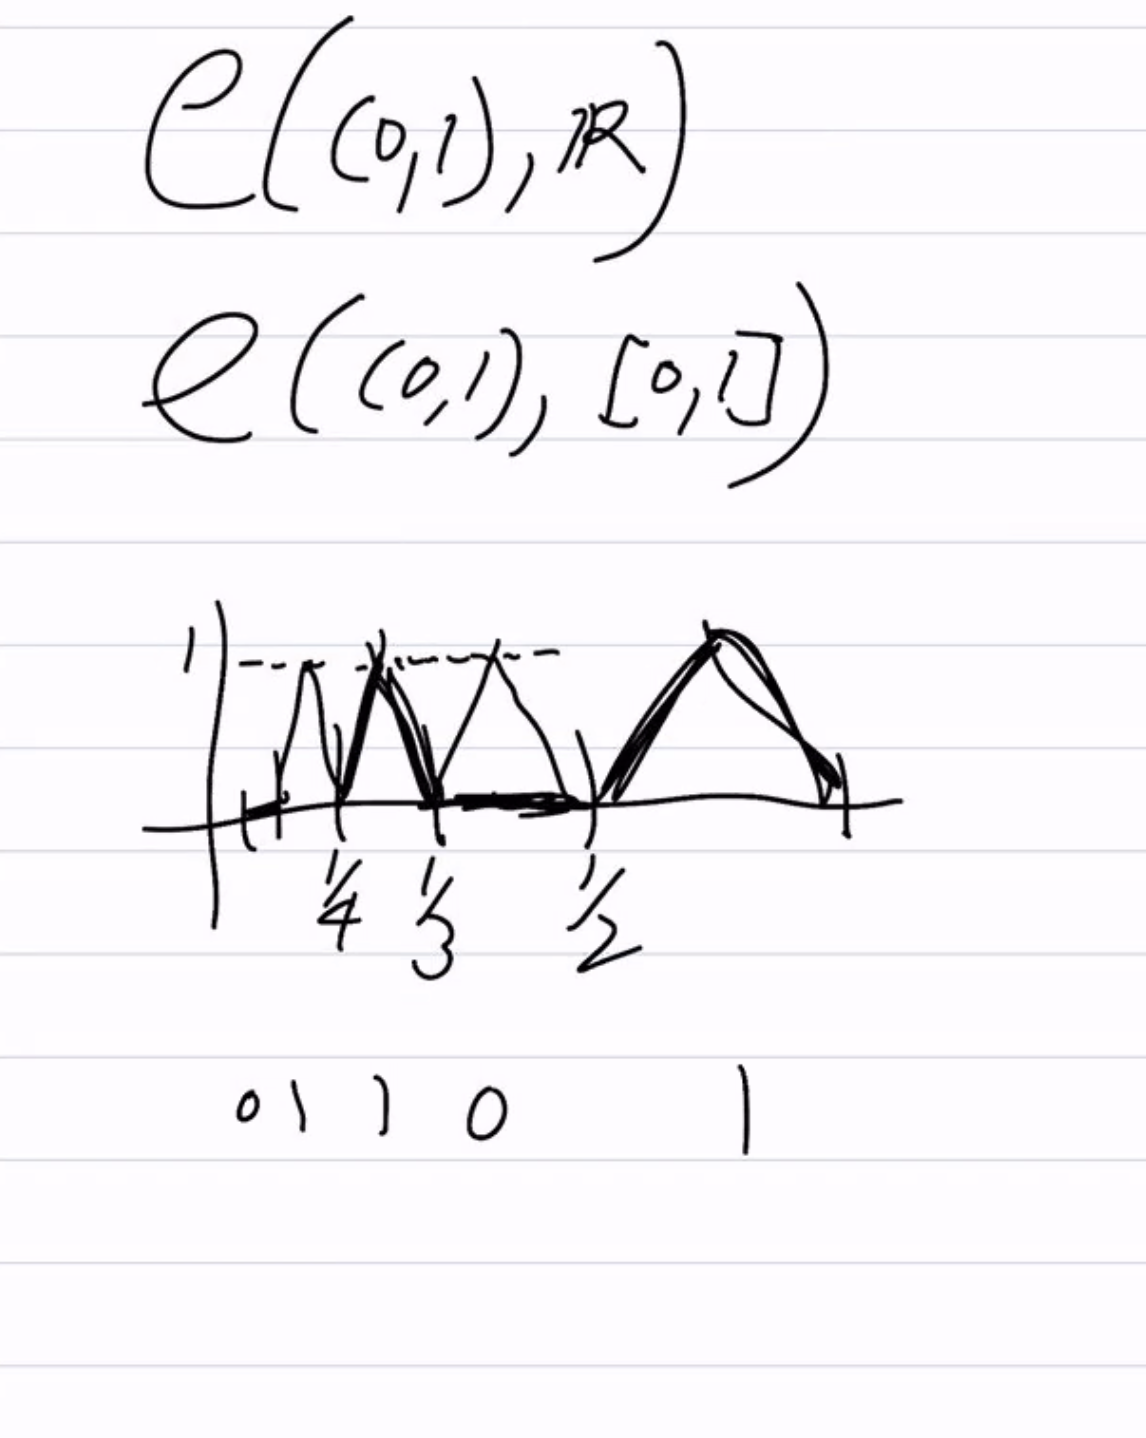
\includegraphics[width=400pt]{img/analysis--berkeley-202a-hw-7459.png}
    \end{mdframed}
  \end{enumerate}


  \newpage
  \begin{mdframed}
    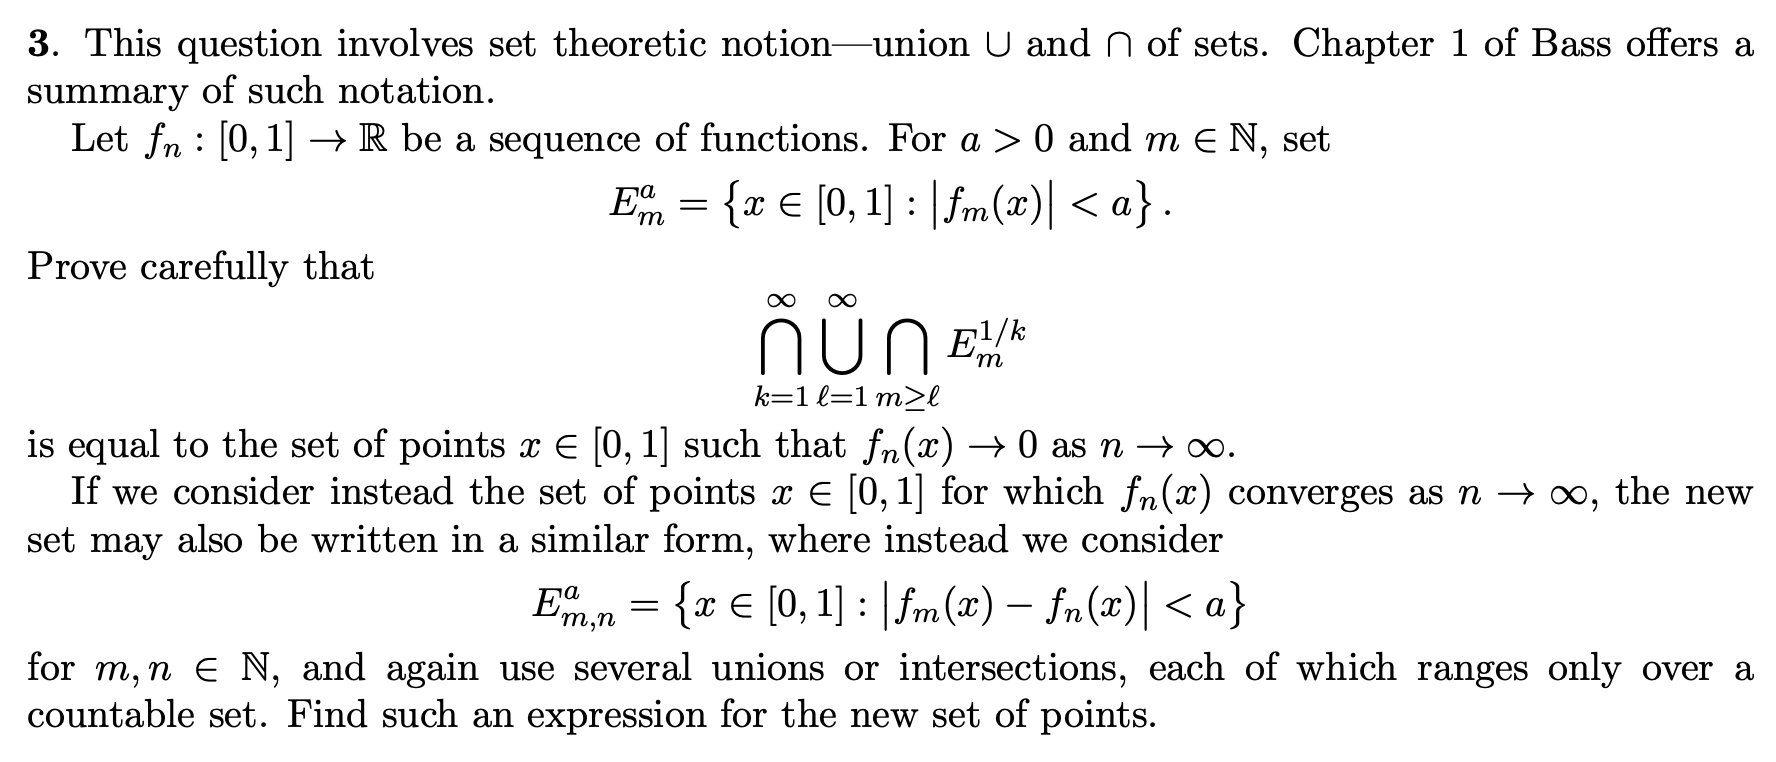
\includegraphics[width=400pt]{img/analysis--berkeley-202a--homework-1-8349.png}
  \end{mdframed}


  \begin{proof}
    Let $E_m^a = \{x \in [0, 1] : |f_m(x) < a|\}$ and let $T = \bigcap_{k=1}^\infty \bigcup_{l=1}^\infty \bigcap_{m > l} E_m^{1/k}$.

    Informally, $E_m^a$ is the set of points for which $f_m$ is within $a$ of zero.

    Let $f_n: [0, 1] \to \R$ be a sequence of functions and let $S \subseteq [0, 1]$ be the set of points $x$
    such that $f_n(x) \to 0$ as $n \to \infty$.

    First we prove that $x \in S \implies x \in T$.

    So let $x \in S$. Then from the definition of limit we have
    \begin{align*}
      &\forall \epsilon>0 ~~~~ \exists l \in \N ~~~~ \forall m \geq l ~~~~  x \in E_m^\epsilon \\
      \iff &\forall \epsilon>0 ~~~~ \exists l \in \N ~~~~                        x \in \bigcap_{m \geq l} E_m^\epsilon \\
      \iff &\forall \epsilon>0 ~~~~                                              x \in \bigcup_{l=1}^\infty \bigcap_{m \geq l} E_m^\epsilon \\
      \iff &                                                              x \in \bigcap_{k=1}^\infty \bigcup_{l=1}^\infty \bigcap_{m \geq l} E_m^{1/k} = T,
    \end{align*}
    as required.

    Secondly we prove that $x \in T \implies x \in S$.

    So let $x \in T$. We have
    \begin{align*}
      x \in \bigcap_{k=1}^\infty \bigcup_{l=1}^\infty \bigcap_{m \geq l} E_m^{1/k},
    \end{align*}
    which is equivalent to the statement
    \begin{align*}
      \forall k>0 ~~~~ \exists l \in \N ~~~~ \forall m \geq l ~~~~  |f_m(x)| < \frac{1}{k}.
    \end{align*}
    Let $\epsilon > 0$ be a real number. Then there exists $k \in \N$ such that $\frac{1}{k} < \epsilon$. Therefore we have
    \begin{align*}
      \forall \epsilon>0 ~~~~ \exists l \in \N ~~~~ \forall m \geq l ~~~~  |f_m(x)| < \epsilon
    \end{align*}
    which is equivalent to $x \in S$, as required.
  \end{proof}

  \begin{proof}
    Let $S \subseteq [0, 1]$ be the set of points $x$ for which $f_n(x)$ converges as $n \to \infty$. Since every
    convergent sequence in the reals is Cauchy, we have that $x \in S$ is equivalent to
    \begin{align*}
      \forall \epsilon > 0 ~~~~ \exists l \in \N ~~~~ \forall m \geq l ~~~~ \forall n \geq l ~~~~ |f_m(x) - f_n(x)| < \epsilon,
    \end{align*}
    which is equivalent to
    \begin{align*}
      \forall \epsilon > 0 ~~~~ x \in \bigcup_{l=1}^\infty \bigcap_{m \geq l} \bigcap_{n \geq l} E_{m,n}^\epsilon.
    \end{align*}
    Therefore, we have that $x \in S$ implies
    \begin{align*}
      x \in \bigcap_{k=1}^\infty \bigcup_{l=1}^\infty \bigcap_{m \geq l} \bigcap_{n \geq l} E_{m,n}^{1/k}.
    \end{align*}
    As before, the reverse implication also holds since, for any given $\epsilon > 0$, we can find a $k \in \N$
    such that $\frac{1}{k} < \epsilon$.
  \end{proof}

  \newpage
  \begin{mdframed}
    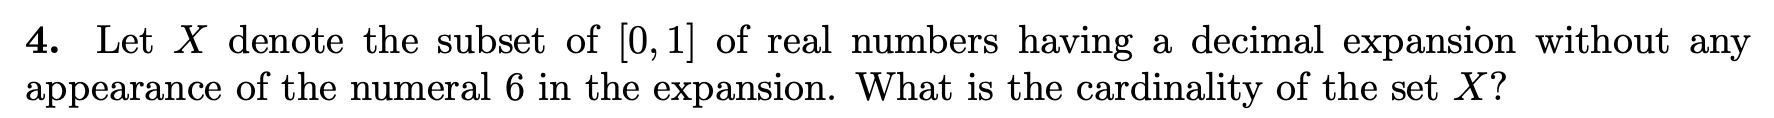
\includegraphics[width=400pt]{img/analysis--berkeley-202a--homework-1-f175.png}
  \end{mdframed}


  \begin{proof}
    Let $X \subset [0, 1]$ be the subset of real numbers without any 6 in their decimal expansion. Let $x \in X$ and let
    \begin{align*}
      d_n(x) =
      \begin{cases}
        0, ~~~~ n\text{-th decimal place of }x \text{ is }0\\
        1, ~~~~ \text{otherwise}.
      \end{cases}
    \end{align*}
    Define $f: X \to [0, 1]$ by setting $f(x)$ equal to the real number whose binary expansion
    is $0.d_1(x)d_2(x)\cdots$.

    Note that for any real number $\om \in [0, 1]$, there exists $x \in X$ such that $f(x) = \om$. To find such
    an $x$, we could for example choose the number whose decimal expansion is equal to the binary expansion
    of $\om$.

    Therefore $f$ is a non-injective surjection from $X$ to the reals in $[0, 1]$, and so the cardinality of $X$
    is at least that of the reals. Since $X \subset \R$ we conclude that the cardinality of $X$ is equal to that
    of the reals.
  \end{proof}

  \newpage
  \begin{mdframed}
    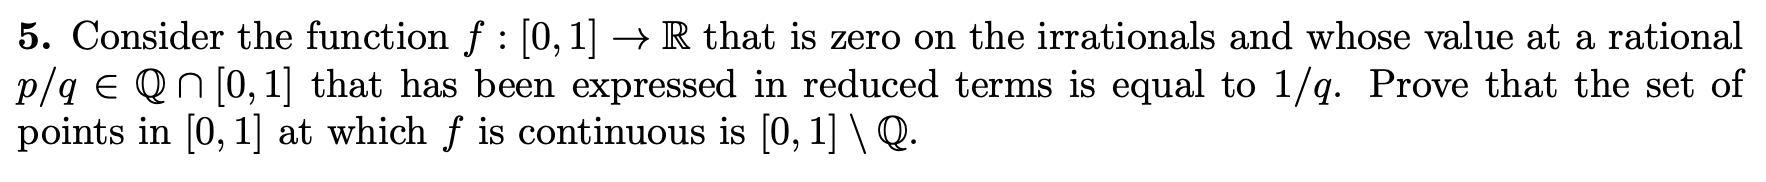
\includegraphics[width=400pt]{img/analysis--berkeley-202a--homework-1-5192.png}
  \end{mdframed}



  \begin{proof}
    Let $X \subseteq [0, 1]$ be the set of points at which $f$ is continuous. We want to show that $f$ is
    continuous at $x$ iff $x$ is not rational.

    Suppose for a contradiction that $f$ is continuous at a rational point $x = p/q$, where $p, q$ are
    non-negative integers. Then $f(x) = 1/q$. But there will always be irrational points within a given
    distance $\delta$ of $x$, now matter how small $\delta$ is, and at such an irrational point $x'$ we
    have $|f(x) - f(x')| = |1/q - 0| = 1/q$. Therefore $f$ is not continuous at $x$ since the definition of
    continuity does not hold for $\epsilon < 1/q$.

    Now let $x$ be irrational, so that $f(x) = 0$. Fix an arbitrary $\epsilon > 0$. We want to show that there
    exists a $\delta$ such that $1/q < \epsilon$ for any rational point $p/q$ lying within $\delta$ of $x$,
    where $p/q$ is in reduced terms. If $\epsilon > 1/2$ then any $\delta$ will work, so
    assume $\epsilon \leq 1/2$. Let $k$ be the largest natural number such that $1/k \geq \epsilon$, let $i$ be
    the largest natural number such that $i/k < x$ and let $j$ be the smallest natural number such
    that $j/k > x$. Then a choice of $\delta = \frac{1}{2}\min\{x - i/k, j/k - x\}$ will work to prove continuity
    of $f$ at irrational $x$.
  \end{proof}


  \begin{mdframed}
    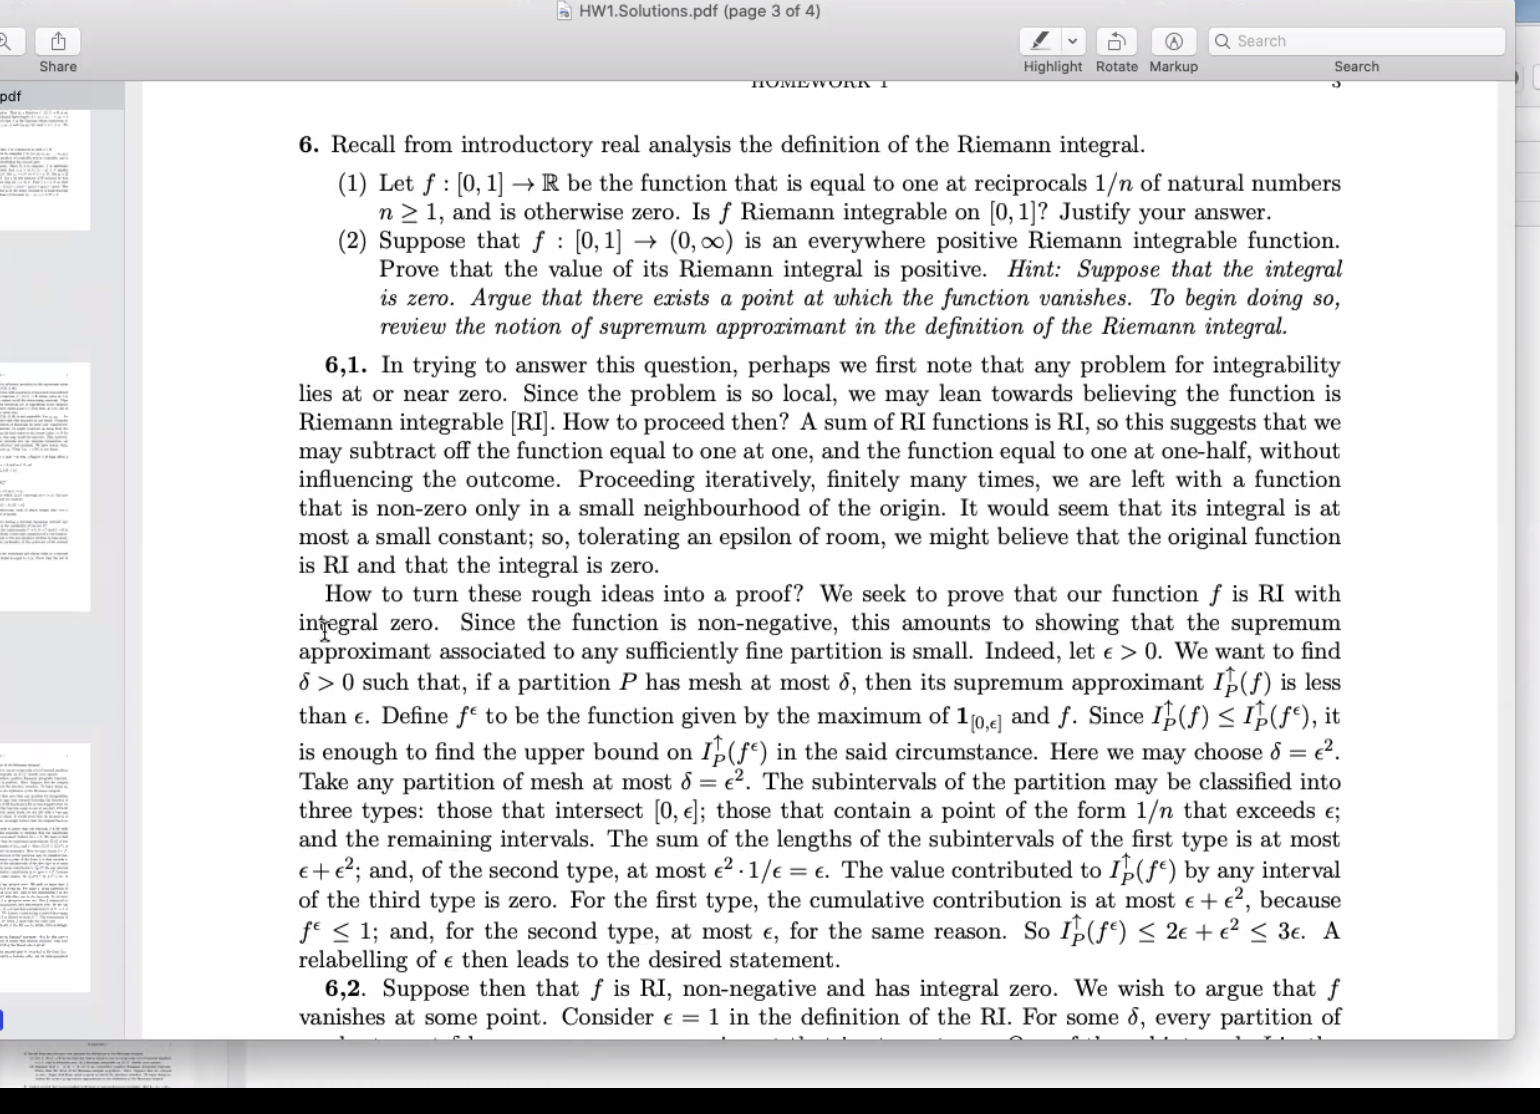
\includegraphics[width=400pt]{img/analysis--berkeley-202a-hw-af4c.png}
  \end{mdframed}


  \begin{mdframed}
    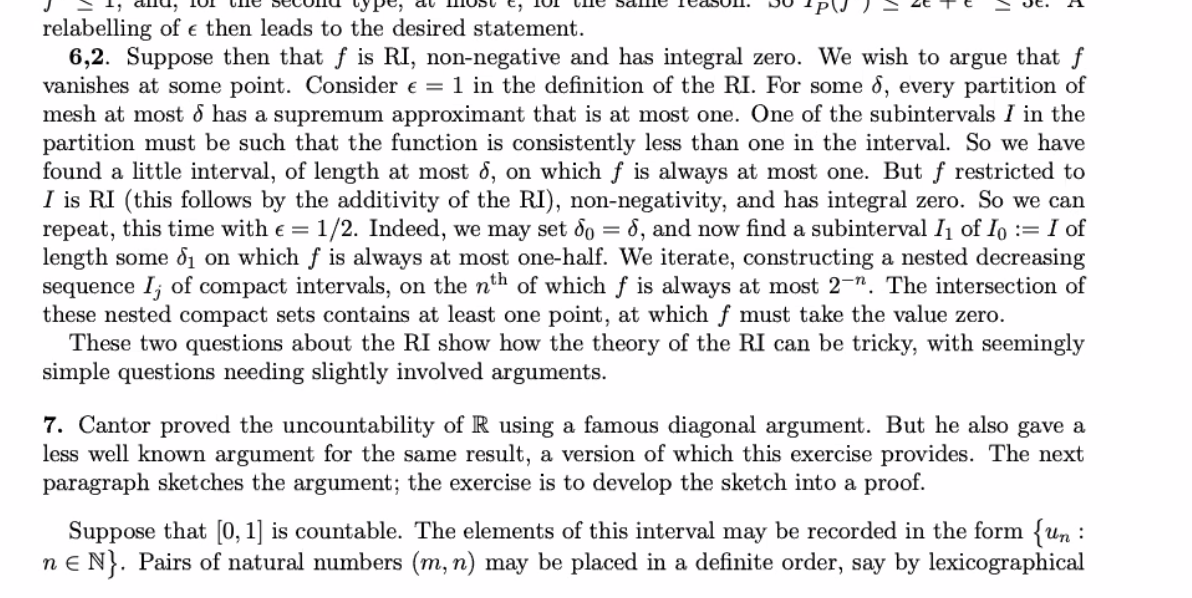
\includegraphics[width=400pt]{img/analysis--berkeley-202a-hw-5fee.png}
  \end{mdframed}




  \newpage
  \begin{mdframed}
    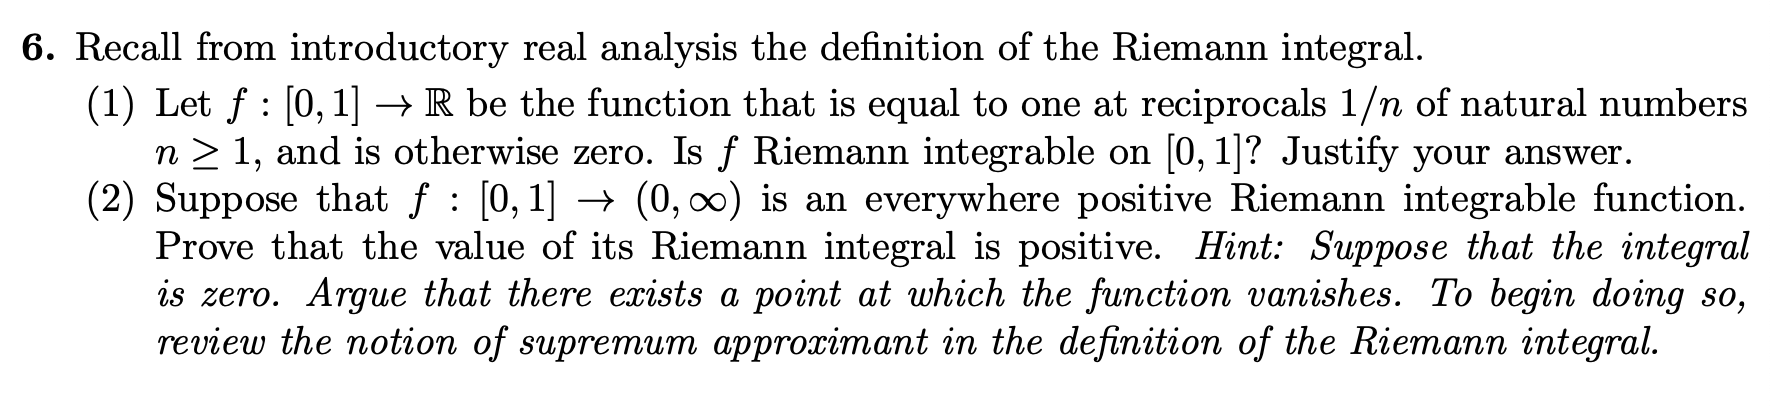
\includegraphics[width=400pt]{img/analysis--berkeley-202a--homework-1-f5e8.png}
  \end{mdframed}





  \begin{definition*}
    $g: [0, 1] \to \R$ is Riemann integrable if
    \begin{align*}
      \sup_{\phi^-} I(\phi^-) = \inf_{\phi^+} I(\phi^+).
    \end{align*}
    Here $\phi^-$ and $\phi^+$ are step functions adapted​ to some
    partition $0 \leq x_1 \leq x_2 \leq \ldots \leq x_{n-1} \leq 1$, such that $\phi(x) = c_i$
    for $x \in (x_{i-1}, x_i)$. $I(\phi)$ is (informally) the area under the step function $\phi$:
    \begin{align*}
      I(\phi) = \sum_{i=1}^n c_i(x_i - x_{i-1}).
    \end{align*}
    And the supremum is over all minorants $\phi^- \leq g$ and the infimum is over all
    majorants $\phi^+ \geq g$, where the length $n$ of the partition is allowed to vary as well as the constant
    values $\{c_1, c_2, \ldots, c_n\}$ of the step function within each segment.
  \end{definition*}

  \begin{enumerate}
  \item
    \begin{claim*}
      The specified function $f$ is not Riemann integrable.
    \end{claim*}

    \begin{proof}
      Consider the first segment of any partition: $(0, x_1)$. No matter how small $x_1$ is, there
      exists $n \in \N$ such that $1/n < x_1$. Therefore for all majorants we have $c_1 \geq 1$ and yet for all
      minorants we have $c_1 \leq 0$. So, when restricted to this first segment, we have $I(\phi^-) > I(\phi^+)$
      for all $\phi^-, \phi^+$ and, since every majorant is elsewhere less than every minorant, it is not
      possible that $\sup_{\phi^-} I(\phi^-) = \inf_{\phi^+} I(\phi^+)$ and hence the Riemann integral is
      undefined.
    \end{proof}

  \item
    \begin{claim*}
      $\int_0^1 f > 0$
    \end{claim*}
    \begin{proof}
      Suppose for a contradiction that $\int_0^1 f = 0$. Fix an arbitrary minorant $\phi^-$, adapted to a
      partition of length $n$. Then we have that $\sum_{i=1}^n c_i(x_i - x_{i-1}) \leq 0$.
      Since $x_i \geq x_{i-1}$ for all $i$, and since $x_0 = 0 < x_n = 1$, it must be the case
      that $x_i - x_{i-1} > 0$ for some $i$, and therefore that $c_i > 0$ for some $i$. Therefore $f$ vanishes at
      at least one point. This contradiction proves that $\int_0^1 f \neq 0$.

      To see that it's not negative, note that for every majorant $\phi^+$ we have $x_i - x_{i-1} \geq 0$
      and $c_i > 0$ for all $i$ and therefore $I(\phi^+) = \sum_{i=1}^n c_i(x_i - x_{i-1}) \geq 0$. Therefore $\int_0^1 f > 0$.
    \end{proof}

  \end{enumerate}

  \newpage
  \begin{mdframed}
    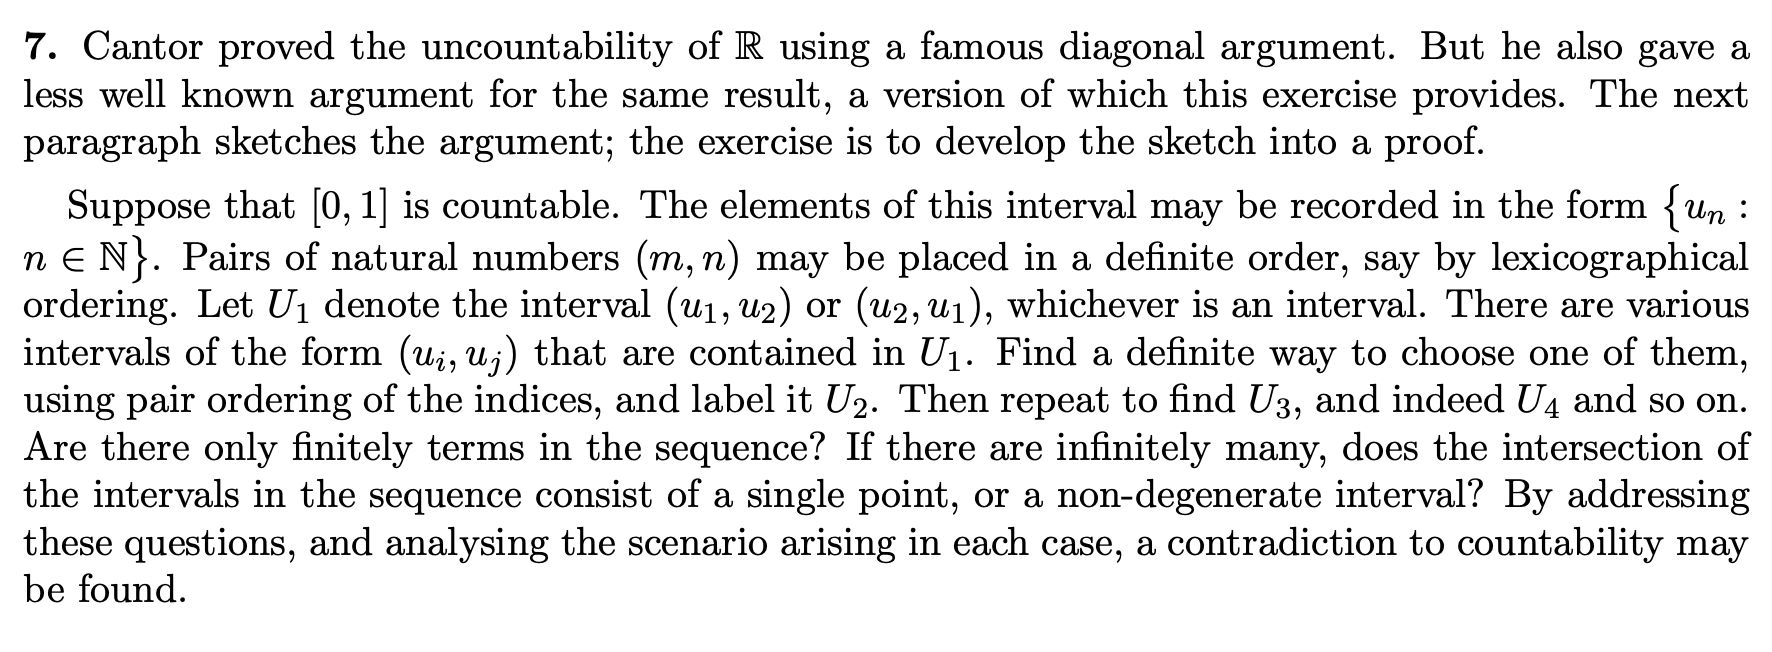
\includegraphics[width=400pt]{img/analysis--berkeley-202a--homework-1-a577.png}
  \end{mdframed}

  \begin{proof}
    Suppose for a contradiction that $[0, 1] \subset \R$ is countable. Fix an enumeration $\{u_n ~|~ n \in \N\}$
    of the elements of $[0, 1]$.

    If $u_1 > u_2$ then relabel them so that $u_1 < u_2$. Set $U_1 = (u_1, u_2)$.

    Continue examining the numbers in the enumeration (starting at $u_3$) until two numbers have been encountered
    that are both in $(u_1, u_2)$. Form an interval from this pair and label it $U_2$. Continue examining the
    numbers in the enumeration until two numbers are encountered that are both in $U_2$; label this
    interval $U_3$. Continue in this fashion indefinitely.

    We will write $(U_{i1}, U_{i2})$ to refer to the endpoints of interval $i$.

    There are two cases:

    \begin{enumerate}
    \item {\bf The process terminates.}\\
      Then there is a last interval $U_L = (U_{L1}, U_{L2})$. It is possible that there is one (but not more than
      one) element $u^*$ of the original enumeration that is present in the interval $U_L$. If that is so, then
      every element of $U_L \setminus \{u^*\}$ is a real number not in the original enumeration; otherwise every
      element of $U_L$ is a real number not in the original enumeration.

    \item {\bf The process does not terminate.}\\
      Note that the sequence of interval lower bounds $(U_{i1})_{i\in\N}$ forms a strictly increasing sequence
      bounded above by $u_2$ and that the sequence of interval upper bounds $(U_{i2})_{i\in\N}$ forms a strictly
      decreasing sequence bounded below by $u_1$. By the Monotone Convergence theorem, both sequences converge:
      let these limits be $\alpha$ and $\beta$ respectively. There are two cases:
      \begin{enumerate}
      \item {\bf $\alpha < \beta$}\\
        Then every element of $(\alpha, \beta)$ is a real number not in the original enumeration.
      \item {\bf $\alpha = \beta$}\\
        Then $\alpha$ is a real number not in the original enumeration.
      \end{enumerate}
    \end{enumerate}

    In all cases, we found a real number that was not present in the original enumeration. But this is a
    contradiction, since the original enumeration contains all real numbers. Therefore no such enumeration exists
    and the real numbers are not countable.
  \end{proof}

\end{comment}


\section*{Math 202a - HW2 - Dan Davison - \texttt{ddavison@berkeley.edu}}

\begin{mdframed}
  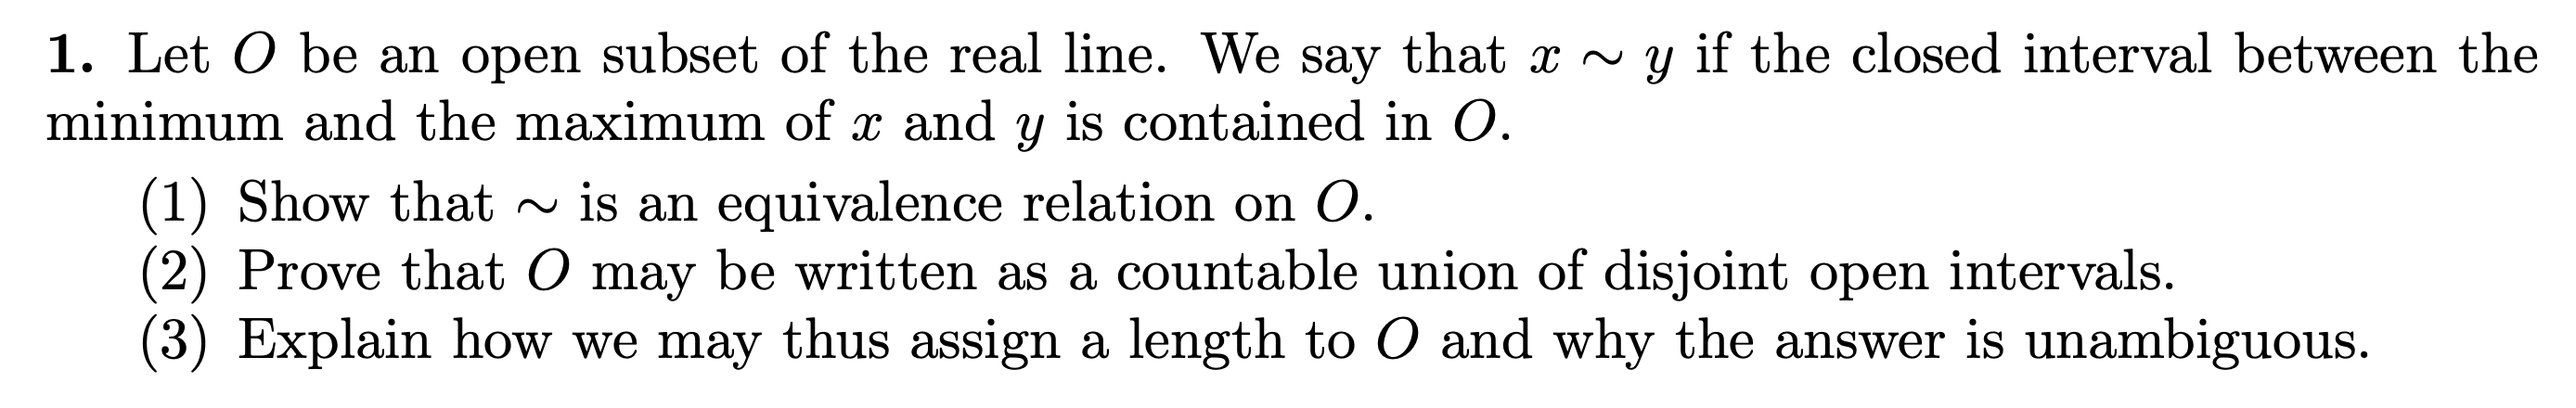
\includegraphics[width=400pt]{img/analysis--berkeley-202a-ebe4.png}
\end{mdframed}

\begin{intuition*}
  $O \subset \R$ is a countable union of disjoint open intervals.

  $x \sim y$ iff $x$ and $y$ are in the same interval.

  The length of $O$ should be the sum of the lengths of the intervals.
\end{intuition*}


\begin{enumerate}[label=(1.\arabic*)]
\item
  \begin{claim*}
    $\sim$ is an equivalence relation on $O$.
  \end{claim*}
  \begin{proof}
    \begin{enumerate}
    \item {\bf Reflexivity}\\
      $x \sim x$ since $[x, x] = \{x\} \subseteq O$.

    \item {\bf Symmetry}\\
      Let $x, y \in \R$ such that $x \sim y$. Then $[\min\{x, y\}, \max\{x, y\}] \subseteq O$.
      Therefore $[\min\{y, x\}, \max\{y, x\}] \subseteq O$. Therefore $y \sim x$.

    \item {\bf Transitivity}\\
      Let $x, y, z \in \R$ such that $x \sim y$ and $y \sim z$. Then $[\min\{x, y\}, \max\{x, y\}] \subseteq O$
      and $[\min\{y, z\}, \max\{y, z\}] \subseteq O$. Therefore $[\min\{x, y\}, \max\{y, z\}] \subseteq O$.
      Therefore $x \sim z$.
    \end{enumerate}
  \end{proof}

\item
  \begin{claim*}
    $O$ may be written as a countable union of disjoint open intervals.
  \end{claim*}

  \begin{proof}
    Let $\mc I = I_1, I_2, \ldots$ be the set of equivalence classes of $O$ under $\sim$.

    Since $\sim$ is an equivalence relation, the elements of $\mc I$ are disjoint and their union is equal
    to $O$.

    We now show that the elements of $I$ are open intervals:

    Let $I \in \mc I$. Note that $I$ has at least two elements since $I$ is an equivalence class. Suppose $I$
    is bounded below and above. Then for any $\epsilon > 0$ there exists $a \in I$ such
    that $a - \inf O < \epsilon$. Note that $[a, x] \subseteq I$ for all $x \in I$ where $a < x$. By a similar
    argument, $[x, b] \subseteq I$ for all $x \in I$ where $b = \sup I$ and $x < b$. It follows from
    transitivity of the equivalence relation that the elements of $\mc I$ are intervals of the
    form $(I_a, I_b)$

    Note that either one of the elements of $I$ has no lower bound, or none do.

    Let $I \in \mc I$.

    We now show that the elements of $\mc I$ are open sets. Let $I \in \mc I$ and suppose for a contradiction
    that $I$ is not open. Then there exists $x \in I$ such that no neighborhood of $x$ is contained within $I$.
    Let $x$ be such a point and let $N(x)$ be a neighborhood of $x$. We claim
    that $N(x) \cap (\R \setminus O) \neq \emptyset$, i.e. that $N(x)$ contains a point outside $O$. [Incomplete]

    We now show that this is a countable union.

    Note that every rational number is in zero or one interval, but not more than one. Furthermore, every
    interval contains at least one rational.

    Therefore there is a non-injective surjection from a subset of the rationals to the set of intervals.

    Therefore the cardinality of the set of intervals is not greater than the cardinality of the rationals.

    Therefore the set of intervals is countable.
  \end{proof}

\item
  \begin{proof}
    We may assign a length $\mu(O)$ to $O$ as follows:

    If $O = \emptyset$ then $\mu(O) := 0$.

    Otherwise, if $O$ is not bounded below, or if $O$ is not bounded above, then $\mu(O) := \infty$.

    Otherwise, if the series $\sum_i |I_i|$ diverges, then $\mu(O) := \infty$.

    Otherwise, $\mu(O) := \sum_i |I_i|$.

    Note that every term of the series is positive. In order for this definition to be unambiguous, the
    value $\mu(O)$ must not depend on the ordering of the series. This is true by the lemma below.
  \end{proof}

  \begin{lemma*}
    Let $\sum_i a_i$ be a series with $a_i > 0$ for all $i$. Then
    \begin{enumerate}
    \item If the series diverges for any ordering of the series, it diverges for all orderings.
    \item If the series converges for any ordering of the series, it converges to the same value for all
      orderings.
    \end{enumerate}
  \end{lemma*}
  \begin{proof}
    A sketch proof of the second statement is as follows: given any $\epsilon > 0$ we can identify a tail of
    the sequence whose sum is less than $\epsilon$. Thus the sum of the series is determined by the finite
    head. The sum of this finite head does not depend on its ordering, by commutativity of addition.
  \end{proof}
\end{enumerate}


\newpage
\begin{mdframed}
  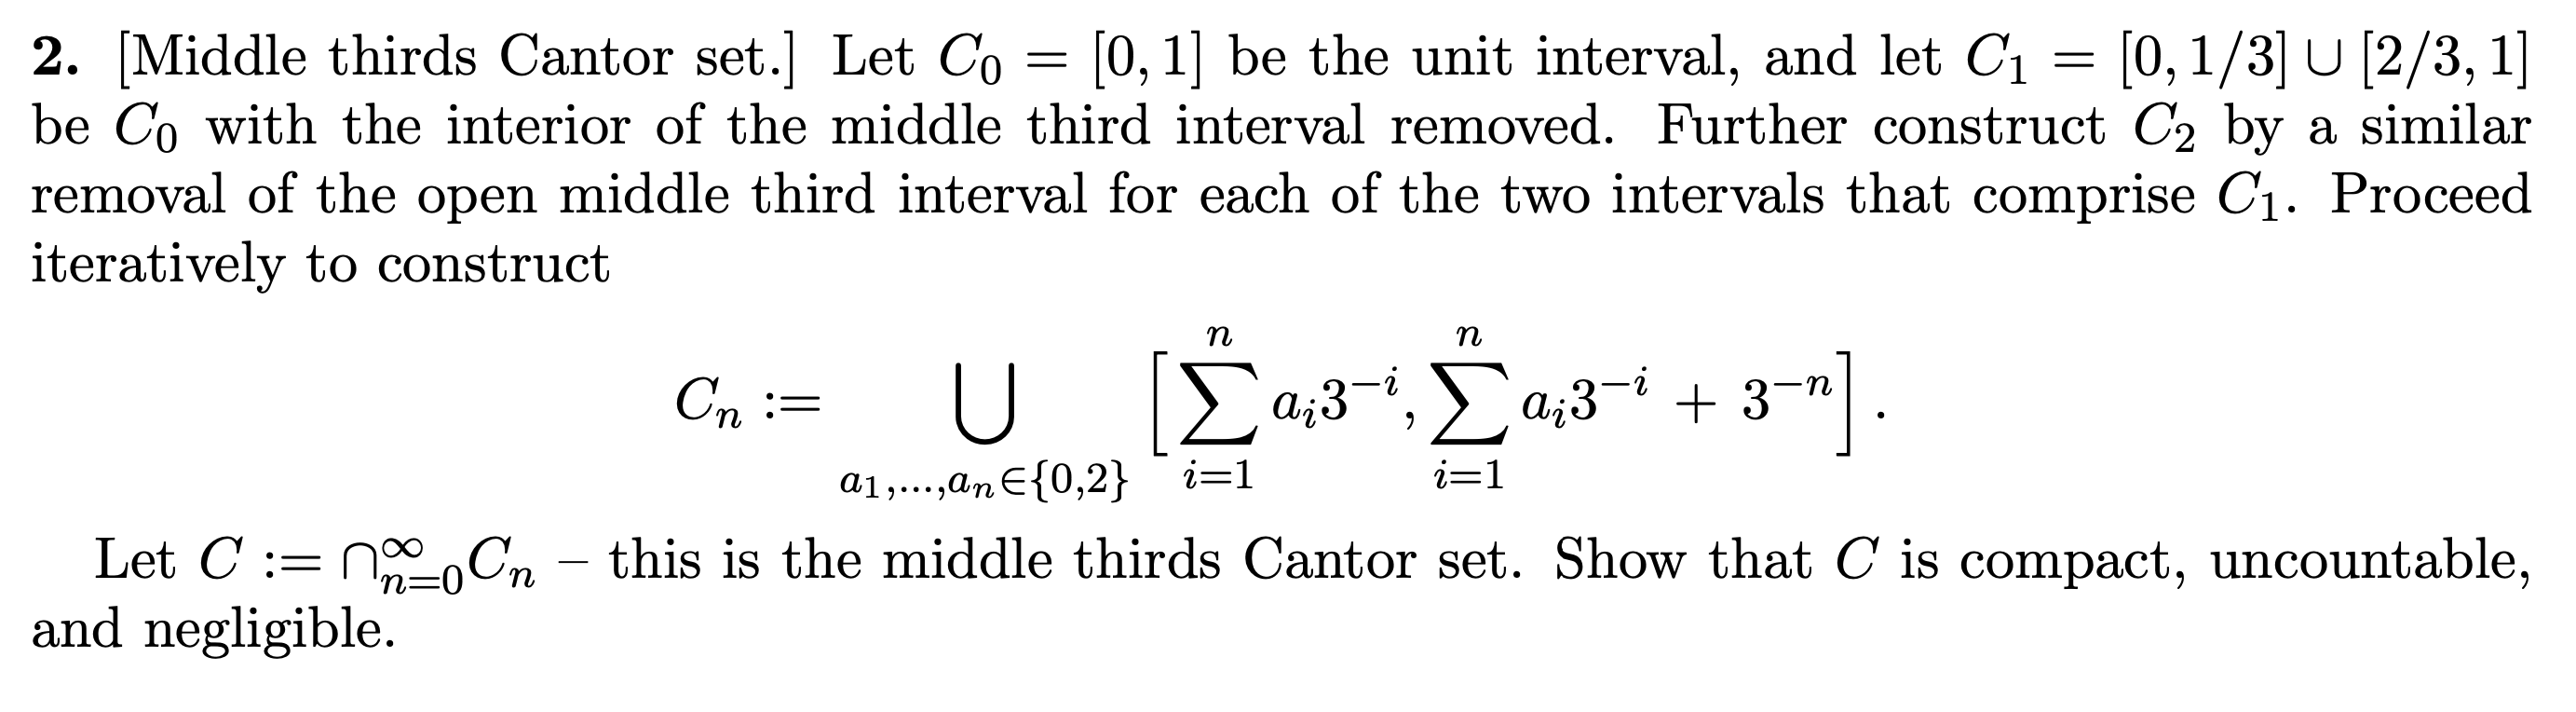
\includegraphics[width=400pt]{img/analysis--berkeley-202a-8d78.png}
\end{mdframed}

\begin{enumerate}[label=(2.\arabic*)]
\item
  \begin{claim*}
    $C$ is compact.
  \end{claim*}
  \begin{proof} \green{DONE}
    Since $C \subset \R$ it suffices to show that $C$ is closed and bounded. Then it follows from the Heine-Borel
    theorem that $C$ is compact.

    $C$ is bounded below by $0$ and above by $1$, since it is constructed by removing points from $[0, 1]$.

    To show that $C$ is closed we may show that $C^c$ is open. Since $C = \bigcap_{n=0}^\infty C_n$, we
    have $C^c = \bigcup_{n=0}^\infty C_n^c$. Note that $C_n$ is a union of closed intervals; therefore $C_n^c$
    is a union of open intervals and therefore open (if an interval contains a neighborhood of each one of its
    points then the union of intervals also contains neighborhoods of those points); therefore $C^c$ is a union
    of open intervals and therefore open. Therefore $C$ is closed.
  \end{proof}

\item
  \begin{claim*}
    $C$ is uncountable.
  \end{claim*}

  \begin{proof}
    Note that $\om \in C$ if and only if the base 3 (ternary) expansion of $\om$ contains no $1$s.

    Consider the map $f:C \to [0, 1]$ defined by the following rule: $f(\om)$ is equal to the real number whose
    binary expansion is formed by substituting every $2$ with a $1$ in the ternary expansion of $\om$.

    This map is a bijection, therefore the cardinality of $C$ is equal to that of $[0, 1]$, therefore $C$ is
    uncountable.
  \end{proof}

\item \begin{claim*}
    $C$ is negligible.
  \end{claim*}

  \begin{proof}
    Fix an arbitrary $\epsilon > 0$. We will show that there exists a countable union of
    intervals $I_1, I_2, \ldots$ that cover $C$ and for which $\sum_k |I_k| < \epsilon$.

    Note that $C_n$ comprises $2^n$ disjoint intervals each of length $3^{-n}$. Therefore the total length
    of $C_n$ is $|C_n| = \big(\frac{2}{3}\big)^n$ and we see that $|C_n| < \epsilon$ for all $n > \Big\lceil\frac{\log\eps}{\log 2/3} \Big\rceil$.

    Let $C = \bigcup_{k=1}^\infty I_k$. We can construct an efficient cover for $C$ as follows:
    for $k \in \{1, 2, \ldots\}$ place an interval of length $2^{-k}$ over $I_k$.

    \red{TODO} Tie this up by giving explicit coordinates for the intervals in the covering.
  \end{proof}

\end{enumerate}

\newpage
\begin{mdframed}
  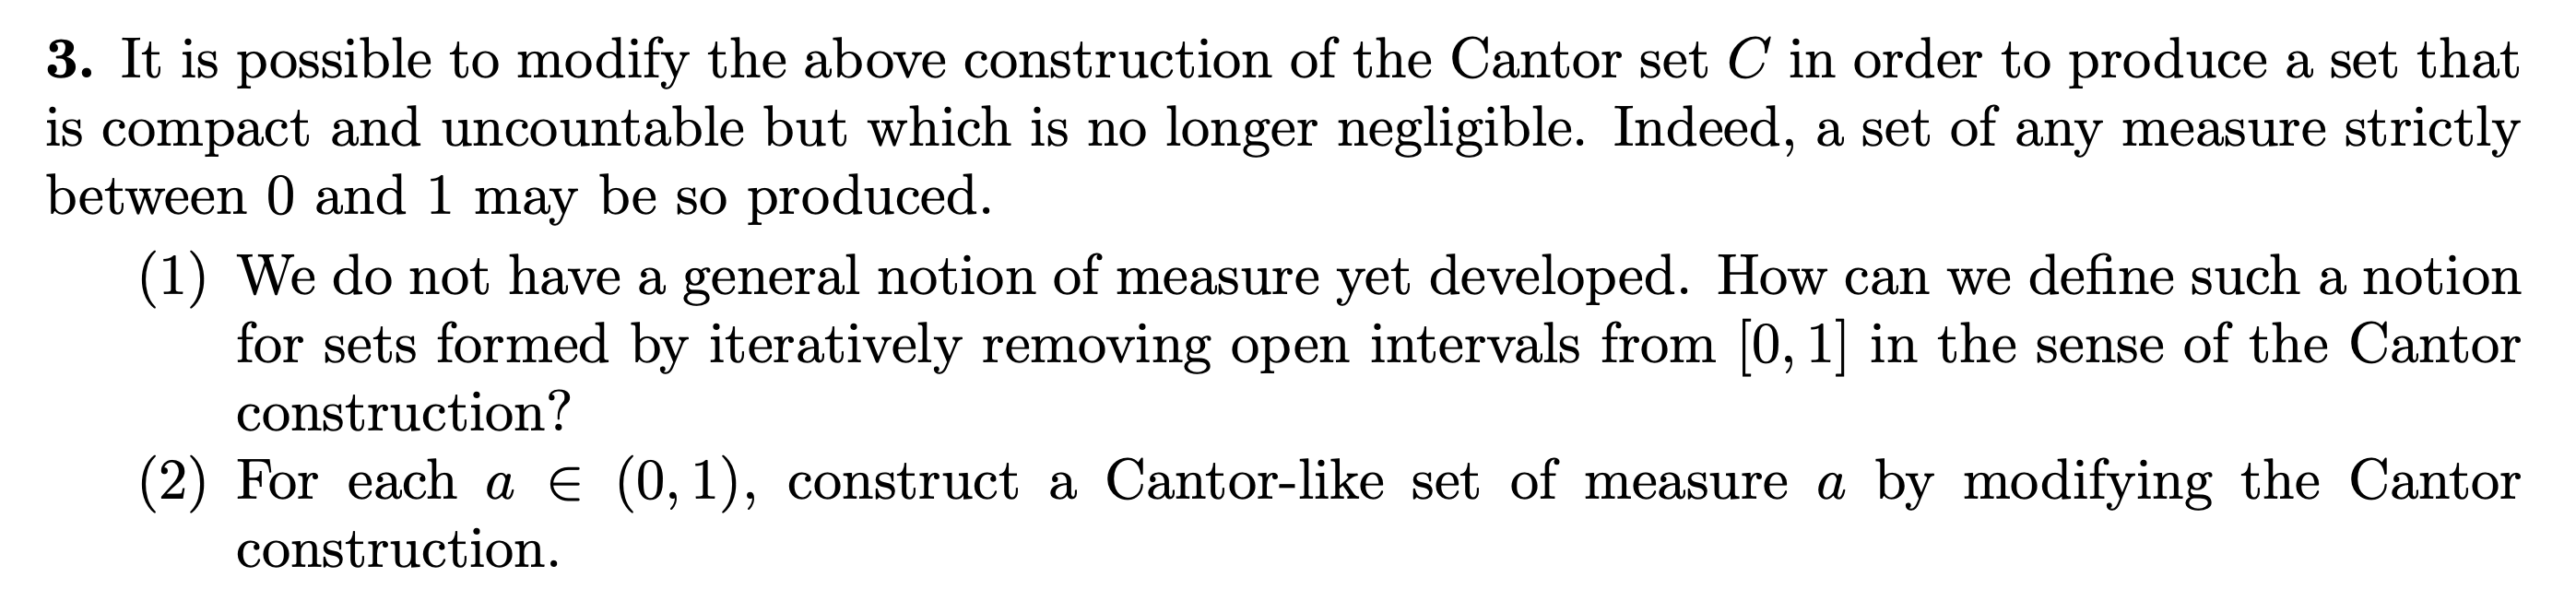
\includegraphics[width=400pt]{img/analysis--berkeley-202a-6b7a.png}
\end{mdframed}

\begin{enumerate}[label=(3.\arabic*)]

\item
  \begin{definition*}
    Let $X$ be a set formed by iteratively removing open intervals from $[0, 1]$. Let $I_1, I_2, \ldots$ be the
    open intervals that were removed in the formation of $X$. Note that these are disjoint, since a point can
    not be removed more than once. Define the measure of $X$ to be $1 - \sum_k |I_k|$.
  \end{definition*}

\item
  \begin{definition*}[Cantor set of measure $a$]
    Let $a \in (0, 1)$. The Cantor set of measure $a$ is formed as follows:

    Instead of removing $1/3$ at each iteration, we will remove a smaller fraction.

    Note that $\sum_{i=1}^\infty \frac{1 - a}{2^i} = 1 - a$. So the algorithm will be the same as the standard
    Cantor set construction except that, instead of removing the middle $1/3$, we remove the
    middle $\frac{1 - a}{2^i}$ of each remaining interval at the $i$-th iteration.
  \end{definition*}

\end{enumerate}



\newpage
\begin{mdframed}
  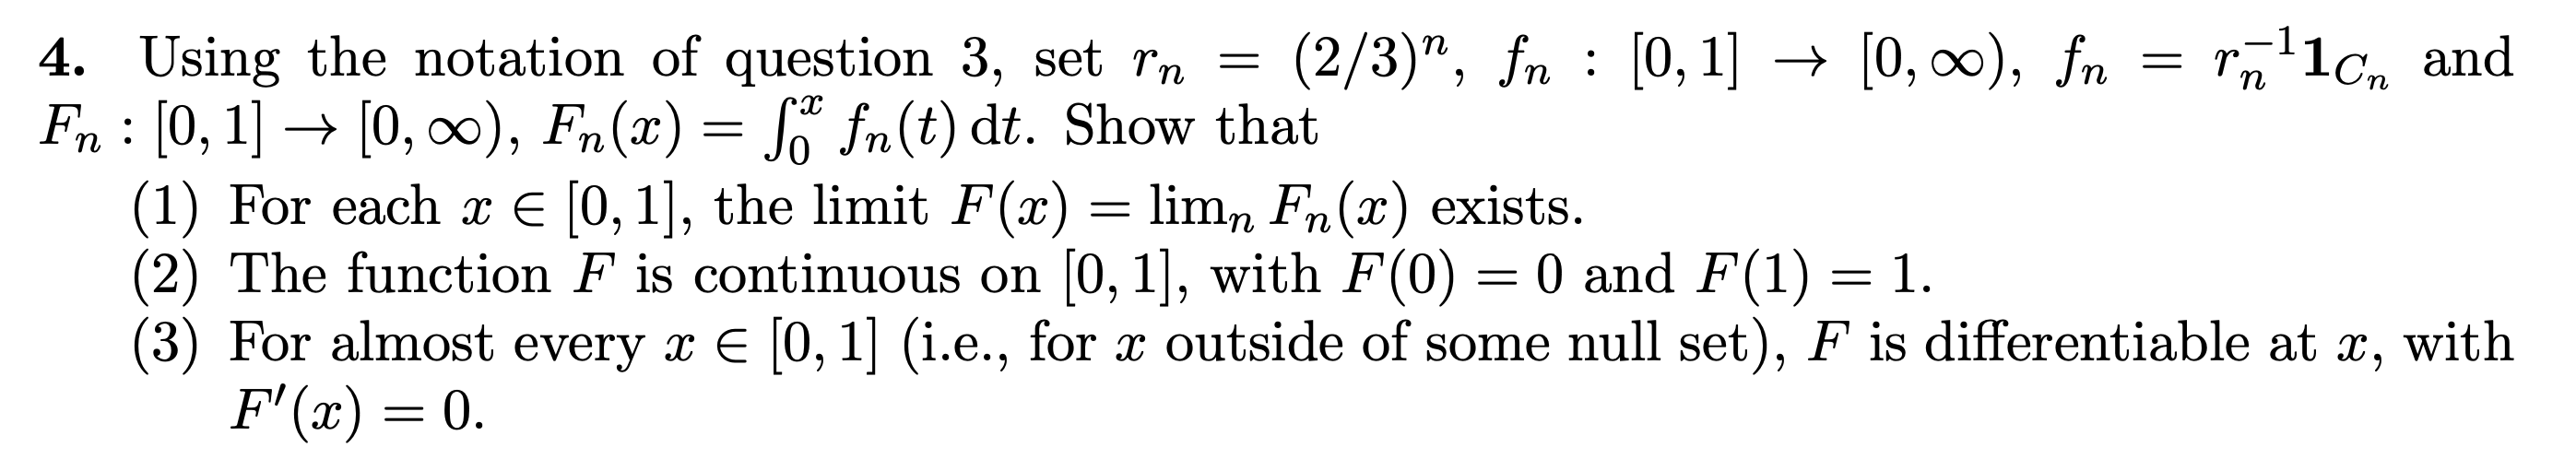
\includegraphics[width=400pt]{img/analysis--berkeley-202a-8ce8.png}
\end{mdframed}

{\bf Some facts:}\\

$C_n$ is a union of $2^n$ intervals, each of length $1/3^n$, therefore the total length is
decreasing: $|C_n| = (2/3)^n$. The function $f_n$ has the value $(3/2)^n$ on each interval in $C_n$ and zero
elsewhere. Therefore $F_n(1) = \(\frac{3}{2}\)^n\(\frac{2}{3}\)^n = 1$ for all $n$.

\begin{enumerate}[label=(4.\arabic*)]

\item
  \begin{lemma*}\label{lemma-4-1-1}
    Let $x \in C^c$. There exists $m$ such that $F_{n+1}(x) = F_n(x)$ for all $n > m$.
  \end{lemma*}
  \begin{proof}
    Let $x \in C^c$. Then there exists $m$ such that for all $n > m$ we have $x \in C_n^c$. Let $m$ be such a
    value and fix an arbitrary $n > m$. We write $C_n$ as a union of $2^n$ closed
    intervals, $C_n = \bigcup_{i=1}^{2^n} [a_i, b_i]$, and let $k = |\{i \in \{1, \ldots, 2^n\} ~:~ b_i < x\}|$
    be the number of these intervals whose right endpoints are less than $x$. We have
    \begin{align*}
      F_n(x) = k\Big(\frac{3}{2}\Big)^n\Big(\frac{1}{3}\Big)^n = \frac{k}{2^n}.
    \end{align*}
    At the next generation, there are $2k$ of these intervals whose right endpoints are less than $x$, and we
    have
    \begin{align*}
      F_{n+1}(x) = 2k\Big(\frac{3}{2}\Big)^{n+1}\Big(\frac{1}{3}\Big)^{n+1} = \frac{k}{2^n}.
    \end{align*}
    Therefore $F_{n+1}(x) = F_n(x)$ for all $n > m$.
  \end{proof}


  \begin{lemma*}\label{lemma-4-1-2}
    Let $[a, b] \subset C$. Then $\int_a^b \big|f_{n+1}(x) - f_n(x)\big| \dx = \frac{1}{3}\frac{1}{2^{n-1}}$.
  \end{lemma*}

  \begin{proof}
    Let $[a, b] \subset C$. For $x$ in the left or right thirds (closed) of this interval we have
    \begin{align*}
      f_{n+1}(x) - f_n(x)
      = \Big(\frac{3}{2}\Big)^{n+1} - \Big(\frac{3}{2}\Big)^{n}
      = \frac{1}{2}\Big(\frac{3}{2}\Big)^n,
    \end{align*}
    and for $x$ in the middle third (open) of this interval we have
    \begin{align*}
      f_{n+1}(x) - f_n(x)
      = -\Big(\frac{3}{2}\Big)^{n}.
    \end{align*}
    Since the interval has length $(1/3)^n$ we have
    \begin{align*}
      \int_a^b \big|f_{n+1}(x) - f_n(x)\big| \dx
      &=  \frac{2}{3}\Big(\frac{1}{3}\Big)^n\frac{1}{2}\Big(\frac{3}{2}\Big)^n
        + \frac{1}{3}\Big(\frac{1}{3}\Big)^n\Big(\frac{3}{2}\Big)^n \\
        % &= \Big(\frac{1}{3}\Big)^n\Big(\frac{3}{2}\Big)^n\Big(\frac{2}{3}\frac{1}{2} + \frac{1}{3}\Big) \\
      &= 2\Big(\frac{1}{3}\Big)^{n+1}\Big(\frac{3}{2}\Big)^n\\
      &= \frac{1}{3}\frac{1}{2^{n-1}}.
    \end{align*}
  \end{proof}

  \begin{claim*}
    For each $x \in [0, 1]$ the limit $F(x) = \lim_{n\to\infty} F_n(x)$ exists.
  \end{claim*}

  \begin{proof}
    We will study the difference $|F_{n+1}(x) - F_n(x)|$ and show that this decreases with $n$ in a way that
    implies that the sequence $F_0(x), F_1(x), \ldots$ is Cauchy for all $x \in [0, 1]$.

    First consider $x \in C^c$. Then from lemma (\ref{lemma-4-1-1}) we have that $F_{n+1}(x) - F_{n}(x) = 0$
    for sufficiently large $n$ and so the sequence is obviously Cauchy.

    Next let $x \in C$ and let $[a, b] \subset C$ be the closed interval containing $x$. Then
    \begin{align*}
      F_{n+1}(x) - F_n(x)
      &= \Big(\int_0^a f_{n+1}(t) \dt + \int_a^x f_{n+1}(t) \dt\Big)
        - \Big(\int_0^a f_{n}(t) \dt   + \int_a^x f_{n}(t) \dt\Big) \\
      &= F_{n+1}(a) - F_{n}(a)
        + \Big(\int_a^x f_{n+1}(t) \dt - \int_a^x f_{n}(t) \dt\Big).
    \end{align*}
    Now, from lemma (\ref{lemma-4-1-1}) we have that $F_{n+1}(x) - F_{n}(x) = 0$ for sufficiently large $n$,
    where $x \in C^c$. But this result also holds for $x$ an endpoint of a closed interval in $C$, since such
    an endpoint is arbitrarily close to a point of $C^c$. Thus we have $F_{n+1}(a) - F_{n}(a) = 0$ and, using
    lemma \ref{lemma-4-1-2},
    \begin{align*}
      \Big|F_{n+1}(x) - F_n(x)\Big|
      &=    \Big|\int_a^x f_{n+1}(t) \dt - f_{n}(t) \dt\Big| \\
      &\leq \int_a^x \big|f_{n+1}(t) \dt - f_{n}(t)\big| \dt \\
      &\leq \int_a^b \big|f_{n+1}(t) \dt - f_{n}(t)\big| \dt \\
      &=    \frac{1}{3}\frac{1}{2^{n-1}} \\
      &<    \frac{1}{2^n}.
    \end{align*}
    In order to show that $F_0(x), F_1(x), \ldots$ is Cauchy, fix $0 < \eps > 1$, let $m \in \N$ be such
    that $\sum_{k=1}^m \frac{1}{2^k} \geq 1 - \eps$, and let $i, j > m$. Then
    \begin{align*}
      \Big|F_i(x) - F_j(x)\Big| \leq \sum_{k=m+1}^\infty \frac{1}{2^k} < \eps.
    \end{align*}
    Therefore the sequence $F_0(x), F_1(x), \ldots$ is Cauchy, and the limit $F(x) = \lim_{n\to\infty} F_n(x)$
    exists for $x \in C$.
  \end{proof}

\item (2) $F$ is piecewise affine, hence continuous.
  \begin{proof}
    There are two cases: $x \in C$ and $x \in C^c$.

    First consider $x \in C^c$. Note that $C^c$ is open, therefore there exists a
    neighborhood $(x - \delta, x + \delta) \subset C^c$. Furthermore, since $f_n(x) = 0$ for all $x \in C^c$,
    we have
    \begin{align*}
      F(x + \delta) - F(x - \delta) = \int_{x-\delta}^{x+\delta}f_n(t) \dt = 0.
    \end{align*}
    Therefore $F$ is continuous at $x \in C^c$, since this choice of $\delta$ works for any $\epsilon$ in the
    definition of continuity.

    Next consider $x \in C$.
  \end{proof}


\item
  \begin{proof}
    For every point $x \in C^c$, $F$ is constant within a neighborhood of $x$. This implies that $F'(x) = 0$
    everywhere except at the endpoints of the intervals that comprise $C$. There are countably many endpoints,
    hence the set of endpoints is a null set (i.e. has measure zero, i.e. is negligible).
  \end{proof}
\end{enumerate}


\newpage
\begin{mdframed}
  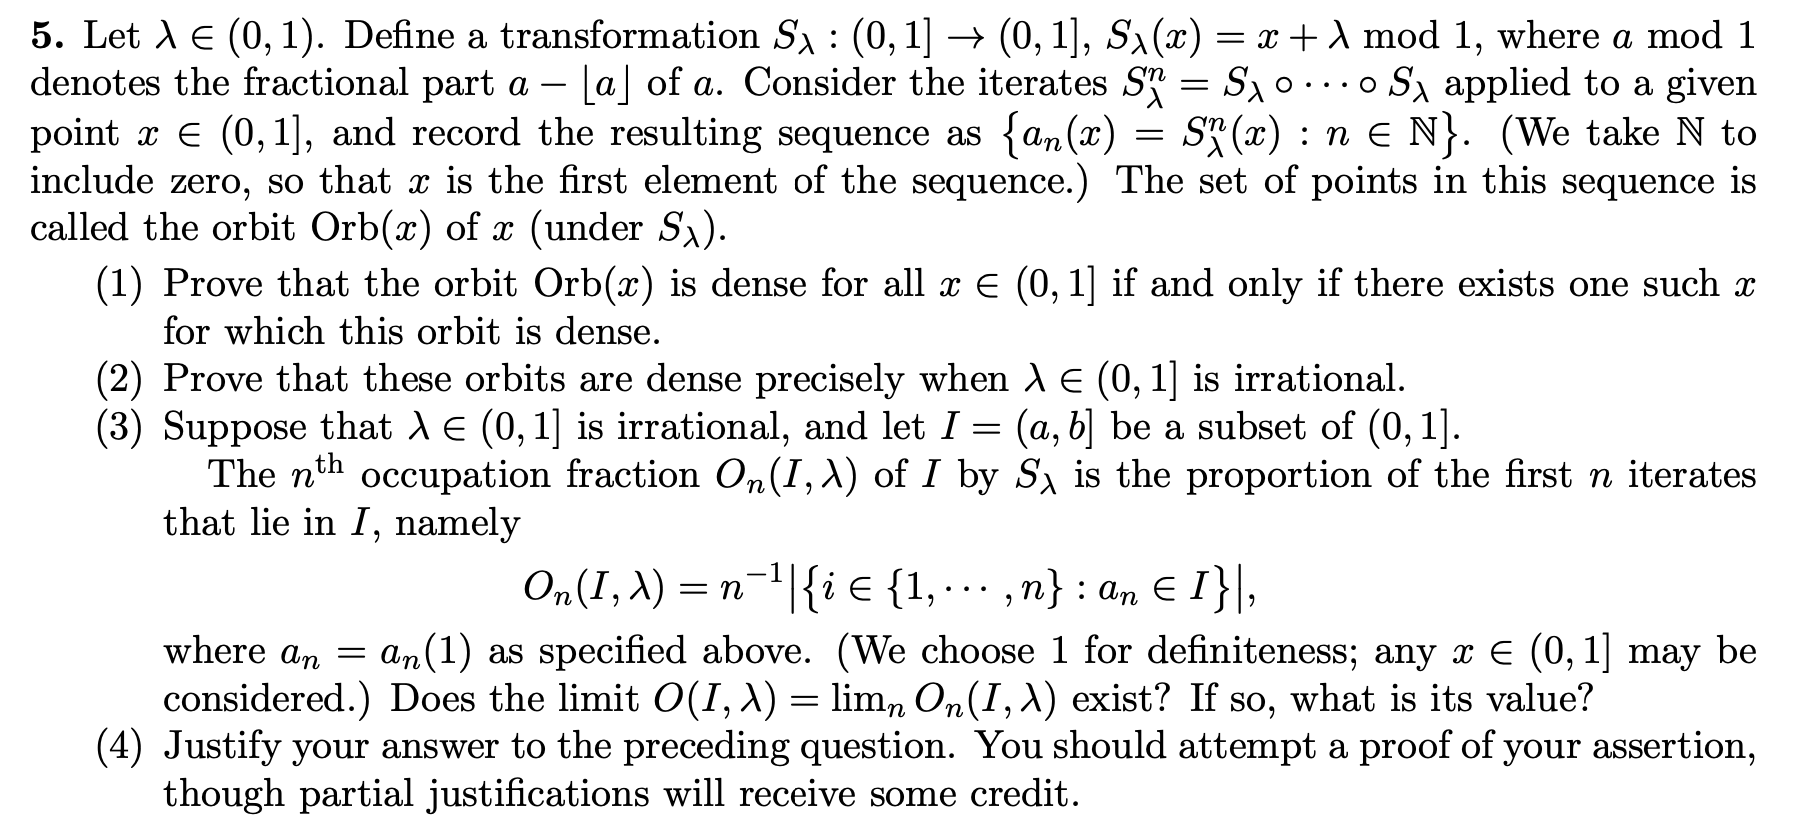
\includegraphics[width=400pt]{img/analysis--berkeley-202a-hw-8c2b.png}
\end{mdframed}

\begin{enumerate}[label=(5.\arabic*)]

\item
  \begin{claim*}
    The orbit $S_{\lambda}(x)$ is dense for all $x \in (0, 1]$ iff there exists an $x$ for which it is dense.
  \end{claim*}
  \begin{proof}
    (running out of time hence informality!)

    Let $x$ be such that $S_\lambda(x)$ is dense. Let $y \neq x$. Since the orbit of $x$ is dense, the sequence
    starting at $x$ will visit a point $y'$ arbitrarily close to $y$. The set of points in the tail of the
    sequence, after visiting $y'$, is the orbit of $y'$. Since the orbit of $x$ is dense, the set of points in
    any tail is also dense, hence $\orb(y')$ is dense.

    But $y'$ differs from $y$ by an arbitrarily small epsilon. Since the transformation is additive, the $i$-th
    element in the sequence starting at $y$ differs from the corresponding element in the sequence starting
    at $y'$ by this same $\eps$. It follows that $\orb(y)$ is dense also.
  \end{proof}

\item
  \begin{claim*}
    The orbits are dense iff $\lambda \in (0, 1]$ is irrational.
  \end{claim*}
  \begin{proof}
    (running out of time hence informality!)

    Let $\lambda \in \Q$. Then $a_n(x) = x + n\lambda \mod 1$.

  \end{proof}
\item
  \begin{definition*}
    The $n$-th occupation fraction of $I$ by $S_\lambda$ is
    \begin{align*}
      O_n(I, \lambda) = \frac{1}{n}\Big|\Big\{i \in \{1, \ldots, n\} ~:~ a_n \in I\Big\}\Big|.
    \end{align*}
  \end{definition*}
  \begin{claim*}
    The occupation fraction has a limiting value: $\lim_{n\to\infty}O_n(I, \lambda) = b - a$.
  \end{claim*}
\item

  \begin{proof}[Proof sketch]
    Focus on the $j$-th digit in the binary expansion of $a_n$, and consider the orbit of that digit alone.
    That's a sequence of $0$s and $1$s that we may interpret as a real number in $[0, 1]$. The claimed result
    would be proved if we can prove the following:

    \begin{enumerate}
    \item The real number corresponding to the sequence visited by the $j$-th digit is normal, for all $j$.
    \item The sequence for digit $j$ becomes (in an appropriate sense) uncorrelated with the sequence for
      digit $k \neq j$.
    \end{enumerate}

    Those two results together would imply that each digit is visiting $0$ and $1$ with equal frequency,
    independently of other digits, and therefore that $a_n$ itself has no tendency to occupy any particular
    dyadic interval more than any other dyadic interval, from which the claimed result follows.

    In order to prove those results, I would investigate the following direction:
    \begin{enumerate}
    \item Note that $\lambda$ is irrational, therefore has a non-repeating binary expansion.

    \item Study the behavior of the binary expansion of $a_n$ under repeated addition of $\lambda$, i.e. with carrying and the mod 1 operation.
    \end{enumerate}
  \end{proof}
\end{enumerate}
